% Copyright 2021 Politecnico di Milano, Italy. Inc. All rights reserved

\documentclass{PoliMi_MasterThesis}

% === Packages and configurations ===
% Configurations
\usepackage{parskip} % For paragraph layout
\usepackage{setspace} % For using single or double spacing
\usepackage{emptypage} % To insert empty pages
\setlength\parindent{0pt} % Indentation
\raggedbottom % Do not stretch empty space to fill the page

% Titles
\usepackage{titlesec}
% \titlespacing{\section}{left spacing}{before spacing}{after spacing}
\titlespacing{\section}{0pt}{3.3ex}{2ex}
\titlespacing{\subsection}{0pt}{3.3ex}{1.65ex}
\titlespacing{\subsubsection}{0pt}{3.3ex}{1ex}
\usepackage{color}

% Language and fonts
\usepackage[english]{babel} % The document is in English  
\usepackage[utf8]{inputenc} % UTF8 encoding
\usepackage[T1]{fontenc} % Font encoding
\usepackage[11pt]{moresize} % Big fonts

% Images
\usepackage{graphicx} % For images
\graphicspath{{./Images/}} % Directory of the images
\usepackage{transparent} % Enables transparent images
\usepackage{eso-pic} % For the background picture on the title page
\usepackage{subfig} % Numbered and caption subfigures using \subfloat.
\usepackage{tikz} % A package for high-quality hand-made figures.
\usetikzlibrary{}
\usepackage{caption} % Coloured captions
\usepackage{xcolor} % Coloured captions
\usepackage{amsthm,thmtools,xcolor} % Coloured "Theorem"
\usepackage{float}

% Math
\usepackage{amsmath}
\usepackage{amsthm}
\usepackage{amssymb}
\usepackage{amsfonts}
\usepackage{bm}
\usepackage[overload]{empheq} % For braced-style systems of equations.
\usepackage{fix-cm} % To override original LaTeX restrictions on sizes

% Tables
\usepackage{tabularx}
\usepackage{longtable} % Tables that can span several pages
\usepackage{colortbl}

% Algorithms
\usepackage{algorithm}
\usepackage{algorithmicx}
\usepackage{algpseudocodex}
\newcommand*\Let[2]{\State #1 $\gets$ #2}
\newcommand*\AAnd{\textbf{ and }}
\newcommand*\AOr{\textbf{ or }}

% Bibliography
\usepackage[colorlinks=true,linkcolor=black,anchorcolor=black,citecolor=black,filecolor=black,menucolor=black,runcolor=black,urlcolor=black]{hyperref} % Adds clickable links at references
\usepackage{cleveref}
\usepackage[square, numbers, sort&compress]{natbib} % Square brackets, citing references with numbers, citations sorted by appearance in the text and compressed
\bibliographystyle{abbrvnat} % You may use a different style adapted to your field

% Other packages
\usepackage{pdfpages} % To include a pdf file
\usepackage{afterpage}
\usepackage{fancyhdr} % For the headers
\fancyhf{}

% Input of configuration file. Do not change config.tex file unless you really know what you are doing. 
% Set the geometric layout of the document
\usepackage{geometry}
\geometry{
  top=3cm,
  left = 1.5cm,
  right = 1.5cm,
  bottom=2cm,
  headheight= 2cm,
  headsep= 0cm,
}
\raggedbottom 

% Create color bluePoli (-> manuale grafica coordinata:  https://www.polimi.it/fileadmin/user_upload/il_Politecnico/grafica-coordinata/2015_05_11_46xy_manuale_grafica_coordinata.pdf)
\definecolor{bluePoli}{cmyk}{0.4,0.1,0,0.4}

% Custom theorem environments
\declaretheoremstyle[
  headfont=\color{bluePoli}\normalfont\bfseries,
  bodyfont=\color{black}\normalfont\itshape,
]{colored}

\captionsetup[figure]{labelfont={color=bluePoli}} % Set colour of the captions
\captionsetup[table]{labelfont={color=bluePoli}} % Set colour of the captions
\captionsetup[algorithm]{labelfont={color=bluePoli}} % Set colour of the captions

\theoremstyle{colored}
\newtheorem{theorem}{Theorem}[section]
\newtheorem{proposition}{Proposition}[section]

% Enhances the features of the standard "table" and "tabular" environments.
\newcommand\T{\rule{0pt}{2.6ex}}
\newcommand\B{\rule[-1.2ex]{0pt}{0pt}}

% Algorithm description
\newcounter{algsubstate}
\renewcommand{\thealgsubstate}{\alph{algsubstate}}
\newenvironment{algsubstates}{
    \setcounter{algsubstate}{0}%
    \renewcommand{\STATE}{%
    \stepcounter{algsubstate}%
    \Statex {\small\thealgsubstate:}\space}
    }{}
    
% Custom theorem environment
\newcolumntype{L}[1]{>{\raggedright\let\newline\\\arraybackslash\hspace{0pt}}m{#1}}
\newcolumntype{C}[1]{>{\centering\let\newline\\\arraybackslash\hspace{0pt}}m{#1}}
\newcolumntype{R}[1]{>{\raggedleft\let\newline\\\arraybackslash\hspace{0pt}}m{#1}}

% Custom itemize environment
\setlist[itemize,1]{label=$\bullet$}
\setlist[itemize,2]{label=$\circ$}
\setlist[itemize,3]{label=$-$}
\setlist{nosep}

% Set separation of columns 
\setlength{\columnsep}{30pt}

% Create command for background pic
\newcommand\BackgroundPic{% Adding background picture
	\put(198,330){
		\parbox[b][\paperheight]{\paperwidth}{%
			\vfill
			\centering
			\transparent{0.4}
			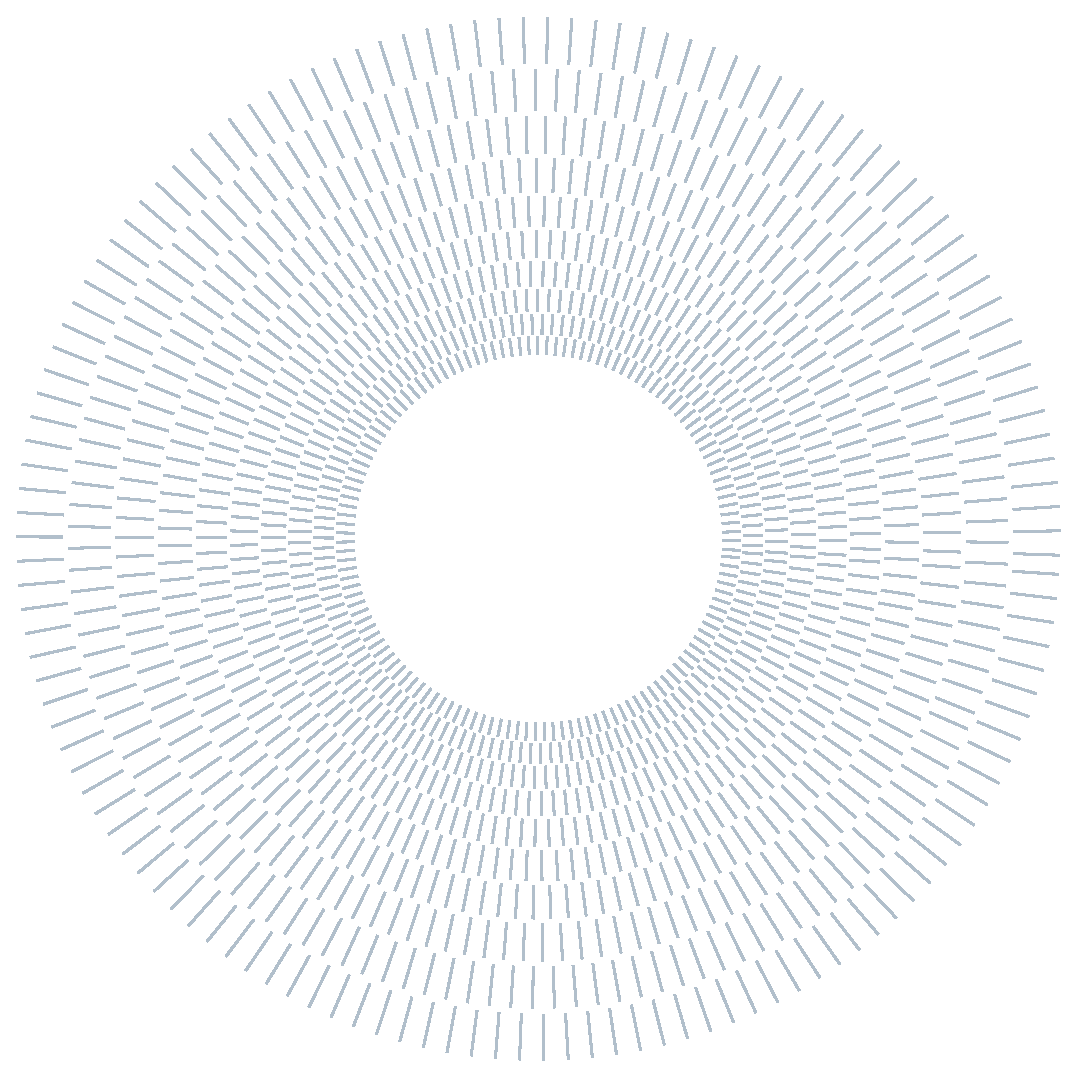
\includegraphics[width=0.7\paperwidth]{raggiera_polimi.eps}%
			\vfill
}}}

% Set indentation
\setlength\parindent{0pt}

% Custom title commands
\titleformat{\section}
{\color{bluePoli}\normalfont\Large\bfseries}
{\color{bluePoli}\thesection.}{1em}{}
\titlespacing*{\section}
{0pt}{2ex}{1ex}

\titleformat{\subsection}
{\color{bluePoli}\normalfont\large\bfseries}
{\color{bluePoli}\thesubsection.}{1em}{}
\titlespacing*{\subsection}
{0pt}{2ex}{1ex}

% Custom headers and footers
\pagestyle{fancy}
\fancyhf{}
      
\fancyfoot{}
\fancyfoot[C]{\thepage} % page
\renewcommand{\headrulewidth}{0mm} % headrule width
\renewcommand{\footrulewidth}{0mm} % footrule width

\makeatletter
\patchcmd{\headrule}{\hrule}{\color{black}\hrule}{}{} % headrule
\patchcmd{\footrule}{\hrule}{\color{black}\hrule}{}{} % footrule
\makeatother

% -> Create the header
\chead[C]{
\centering
\begin{tcolorbox}[arc=0pt, boxrule=0pt, colback=bluePoli!60, width=\textwidth, colupper=white]
    \textsc{\textbf{Executive summary}} \hfill \textsc{\textbf{\author}} 
\end{tcolorbox}
}


% === Start of document ===

\begin{document}

\fancypagestyle{plain}{
\fancyhf{} % Clear all header and footer fields
\fancyhead[RO,RE]{\thepage} %RO=right odd, RE=right even
\renewcommand{\headrulewidth}{0pt}
\renewcommand{\footrulewidth}{0pt}}


% === Title page ===
\pagestyle{empty} % No page numbers
\frontmatter % Use roman page numbering style (i, ii, iii, iv...) for the preamble pages

\puttitle{
	title=Ray Distribution Aware Heuristics for Bounding Volume Hierarchies Construction,
	name=Lapo Falcone,
	course=Computer Science and Engineering,
	ID  = 996089,
	advisor= Prof. Marco Gribaudo,
	academicyear={2023-24}
}


% === Preamble ===
\startpreamble
\setcounter{page}{1} % Set page counter to 1

% Abstract
\chapter*{Abstract} 
Abstract
\\
\\
\textbf{Keywords:} here, the keywords, of your thesis

% Abstract in Italian
\chapter*{Abstract in lingua italiana}
Abstract Italiano
\\
\\
\textbf{Parole chiave:} qui, vanno, le parole chiave, della tesi


% === Table of contents ===
\thispagestyle{empty}
\tableofcontents % Table of contents 
\thispagestyle{empty}
\cleardoublepage

\addtocontents{toc}{\vspace{2em}} % Add a gap in the Contents, for aesthetics
\mainmatter % Begin numeric (1,2,3...) page numbering


% === Intro ===
\chapter*{Introduction}
Intro \cite{meister2021survey}


% === Chapter 1 ===
\chapter{Chapter one}
\label{ch:chapter_one}
Chapter 1


% === Chapter 2 ... ===
\chapter{Chapter two}
Chapter 2


% === Bibliography ===
\addtocontents{toc}{\vspace{2em}} % Add a gap in the Contents, for aesthetics
\bibliography{Bibliography} % The references information are stored in the file named "Bibliography.bib"


% === Appendices ===
\cleardoublepage
\addtocontents{toc}{\vspace{2em}} % Add a gap in the Contents, for aesthetics
\appendix

\chapter{Collision and Culling Algorithms}
\section{Ray-AABB Intersection} \label{sec:ray_box_intersection}
The algorithm we used to detect intersections between a ray and an AABB is the branchless slab algorithm \cite{ray_box_intersection}.

Given a ray in the form: $r(t) = O + t\cdot d$, where $O$ is the origin and $d$ the direction, the main idea of the algorithm is to find the 2 values of $t$ ($\overline{t_1}$ and $\overline{t_2}$) such that $r(\overline{t_{1,2}})$ are the points where the ray intersects the AABB.

Since the object to intersect the ray with is an axis-aligned bounding box in the min-max form, the algorithm can proceed one dimension at a time:
\begin{enumerate}
	\item First, it finds the intersection points of the ray with the planes parallel to the $yz$ plane, and sorts them in an ascending order with reference to the corresponding $\overline{t_{1,2}}$ values. We call the point with the smallest $\overline{t}$ value the \textit{closest}, and the other one the $\overline{furthest}$.
	\item Then it does the same with the $xz$ plane:
	\begin{itemize}
		\item As closest intersection point, it keeps the furthest between the 2 closest intersection points found so far (the one with the $yz$ plane and the one with the $xz$ plane).
		\item As furthest intersection point, it keeps the closest between the 2 furthest intersection points found so far.
	\end{itemize}
	\item Then it does the same with the $xy$ plane.
	\item Finally, an intersection is detected only in the case where the furthest intersection point actually has an associated $\overline{t}$ value bigger than the one of the closest point found by the algorithm.
	\item The returned $\overline{t}$ value is the smaller one, as long as it is greater or equal to 0; otherwise it means that the origin of the ray is inside the AABB, and one of the intersection points is \textit{behind} the ray origin.
\end{enumerate}
	
\begin{figure}[H]
    \centering
    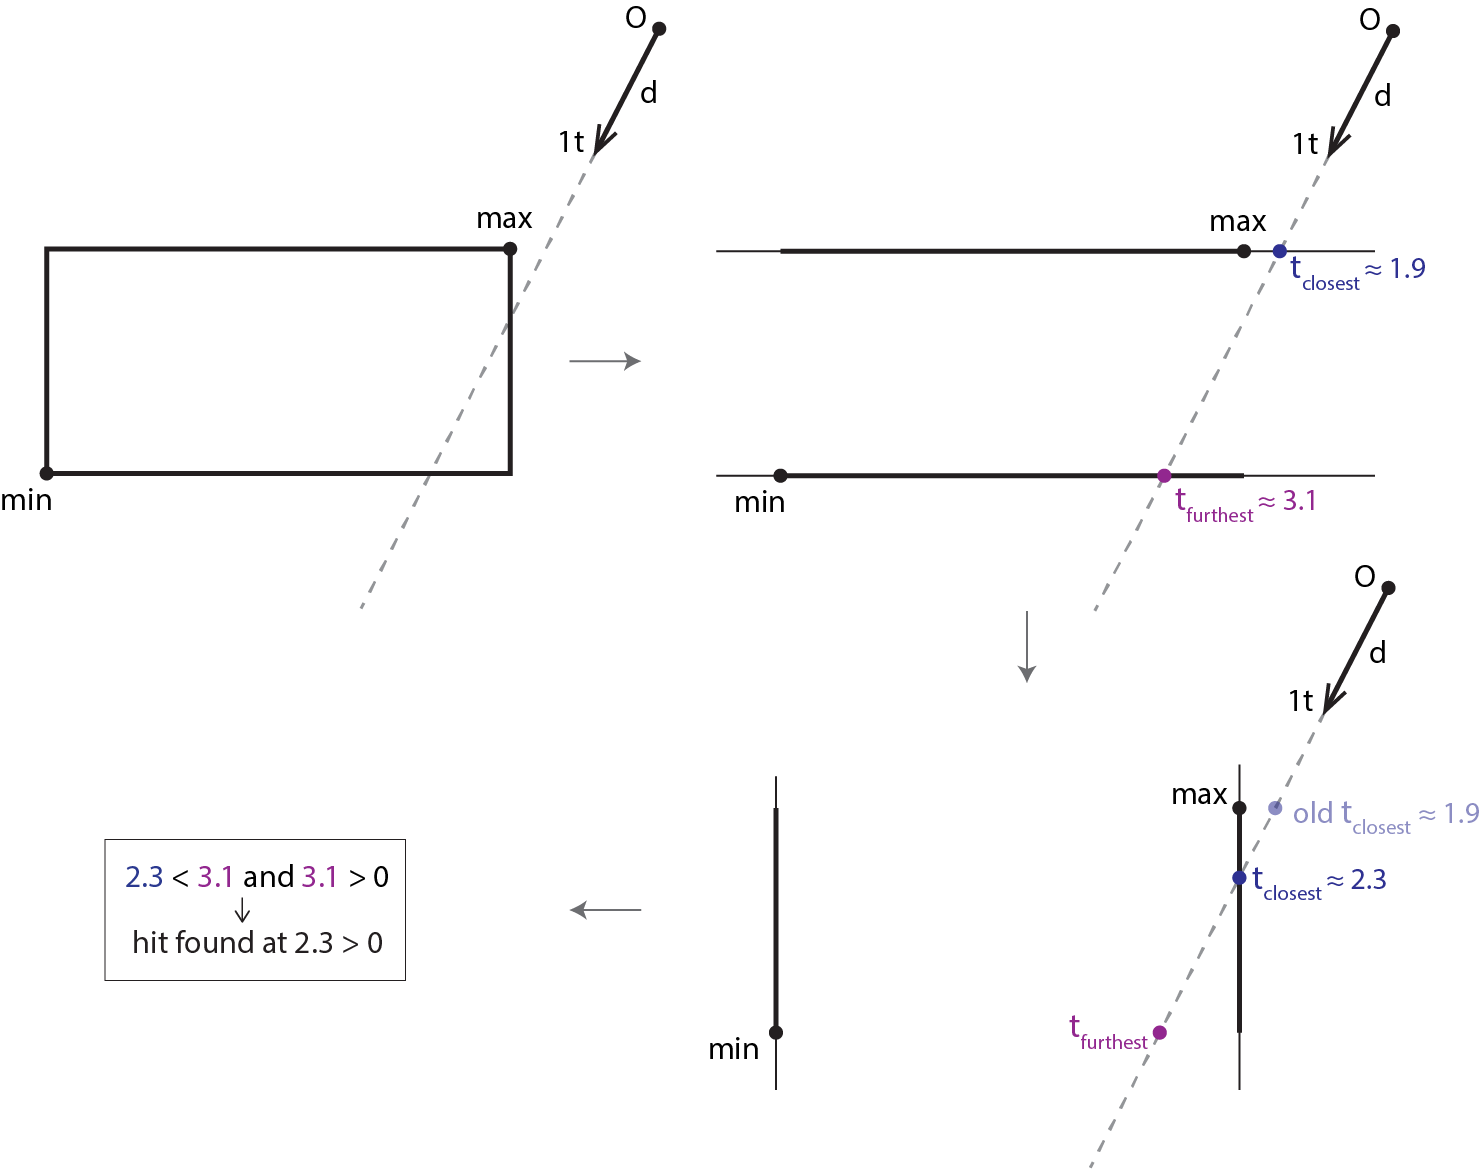
\includegraphics[width=\textwidth]{Images/ray_aabb_intersection.png}
    \caption{Visual representation of the presented algorithm in 2 dimensions. An interactive simulation of this algorithm can be found at: \url{https://www.geogebra.org/m/np3tnjvb}.}
    \label{fig:ray_aabb_intersection}
\end{figure}

\begin{algorithm}[H]
	\caption{Ray-AABB branchless slab intersection algorithm in 3 dimensions}
	\begin{algorithmic}[1]
		\Function{Intersect}{$ray, aabb$}
		\Let {$t1_x$}{$\frac{aabb.min.x - ray.origin.x}{ray.direction.x}$} \Comment{yz plane}
		\Let {$t2_x$}{$\frac{aabb.max.x - ray.origin.x}{ray.direction.x}$}
		\Let {$tMin$}{$min(t1_x, t2_x)$}
		\Let {$tMax$}{$max(t1_x, t2_x)$}
		\Let {$t1_y$}{$\frac{aabb.min.y - ray.origin.y}{ray.direction.y}$} \Comment{xz plane}
		\Let {$t2_y$}{$\frac{aabb.max.y - ray.origin.y}{ray.direction.y}$}
		\Let {$tMin$}{$ max(tMin, min(t1_y, t2_y))$}
		\Let {$tMax$}{$ min(tMax, max(t1_y, t2_y))$}
		\Let {$t1_z$}{$\frac{aabb.min.z - ray.origin.z}{ray.direction.z}$} \Comment{xy plane}
		\Let {$t2_z$}{$\frac{aabb.max.z - ray.origin.z}{ray.direction.z}$}
		\Let {$tMin$}{$max(tMin, min(t1_z, t2_z))$}
		\Let {$tMax$}{$min(tMax, max(t1_z, t2_z))$}
		\Let {$areColliding$}{$tMax > tMin$ \AAnd $tMax \geq 0$}
		\Let {$collisionDist$}{$tMin < 0 \: ? \: tMax \: : \: tMin$}
		\State \Return $\langle areColliding, collisionDist \rangle$
		\EndFunction
	\end{algorithmic}
\end{algorithm} 

It is interesting to note how, under the floating-point IEEE 754 standard, the algorithm also works when it is not possible to find an intersection point along a certain axis (i.e. when the ray is parallel to certain planes). Indeed, in such cases, the values $\overline{t_{1,2}}$ will be $\pm \infty$, and the comparisons will still be well defined.

\section{Ray-Plane Intersection} \label{sec:ray_plane_intersection}
For ray-plane intersection we decided to use this algorithm presented in the educational portal of the SIGGRAPH conference \cite{ray_plane_intersection}.

Given a ray in the form: $r(t) = O + t\cdot d$, where $O$ is the origin and $d$ the direction, and a plane whose normal $n$ and a point $P$ are known, we first check whether the plane and the ray are parallel, in which case no intersection can be found.

Then, if they are not parallel, we obtain the analytic form of the 3-dimensional plane: 
\begin{align*}
	A\cdot x + B\cdot y + C\cdot z + D = 0
\end{align*}
In particular, we know a point $P$ that is part of the plane, therefore we can obtain the $D$ parameter:
\begin{align*}
&A\cdot P_x + B\cdot P_y + C\cdot P_z + D = 0\\
\implies& D = -(A\cdot P_x + B\cdot P_y + C\cdot P_z)
\end{align*}
By definition, the vector formed by the parameters $[A,B,C]$ is perpendicular to the plane, therefore:
\begin{align*}
&D = -(n_x\cdot P_x + n_y\cdot P_y + n_z\cdot P_z)\\
\implies& D = -\langle n \cdot P \rangle
\end{align*}
Now that we have the parametric equation of the plane, we can force a point of the plane to also be a point of the ray: 
\begin{align*}
	&A\cdot r(t)_x + B\cdot r(t)_y + C\cdot r(t)_z + D = 0\\
	\implies& A\cdot (O_x + t\cdot d_x) + B\cdot (O_y + t\cdot d_y) + C\cdot (O_z + t\cdot d_z) + D = 0\\
	\implies& t = \frac{-\langle n\cdot O \rangle + D}{\langle n\cdot d \rangle}
\end{align*}
Finally, if the found $\overline{t}$ value is negative, it means that the intersection point between the ray and the plane is \textit{behind} the ray origin, therefore no intersection is found. Else the ray intersects the plane at point $r(\overline{t})$.

\begin{algorithm}[H]
	\caption{Ray-plane intersection algorithm}
	\begin{algorithmic}[1]
		\Function{Intersect}{$ray, plane$}
		\Let{$d$}{$ray.direction$}
		\Let{$O$}{$ray.origin$}
		\Let{$n$}{$plane.normal$}
		\Let{$P$}{$plane.point$}
		\If{$\langle n\cdot d \rangle = 0$} \Comment{Ray is parallel to plane}
			\State \Return $\langle false, \_ \rangle$
		\EndIf
		\Let{$D$}{$-\langle n\cdot P \rangle$}
		\Let{$t$}{$\frac{-\langle n\cdot O \rangle}{\langle n\cdot d \rangle}$}
		\If{$t<0$} \Comment{Intersection point is \textit{behind} ray origin}
			\State \Return $\langle false, \_ \rangle$
		\Else
			\State \Return $\langle true, t \rangle$
		\EndIf
		\EndFunction
	\end{algorithmic}
\end{algorithm} 

\section{Ray-Triangle Intersection} \label{sec:ray_triangle_intersection}
Once we have algorithms to check for ray-plane intersection (\ref{sec:ray_plane_intersection}) and for a point inside a 2D convex hull (\ref{sec:point_inside_2dHull}), we can combine them to check if a ray intersects a triangle and to compute the coordinates of the intersection point:

\begin{enumerate}
	\item Build a plane that has as normal the normal to the triangle, and as point any vertex of the triangle;
	\item Use the ray-plane intersection algorithm (\ref{sec:ray_plane_intersection}) to find the coordinates of the point where the ray and the plane collide (if any);
	\item Use the point inside 2D convex hull test (\ref{sec:point_inside_2dHull}) to determine if the intersection point is inside the triangle.
\end{enumerate}

\section{AABB-AABB Intersection} \label{sec:aabb_aabb_intersection}
To detect a collision between 2 axis-aligned bounding boxes in the min-max form, it is sufficient to check that there is an overlap between them in all 3 dimensions. By naming the 2 AABBs as $A$ and $B$ we get:
\begin{subequations}
	\begin{align*}[left=\empheqlbrace]
		A.min_x \leq& B.max_x \\
		A.max_x \geq& B.min_x \\
		A.min_y \leq& B.max_y \\
		A.max_y \geq& B.min_y \\
		A.min_z \leq& B.max_z \\
		A.max_z \geq& B.min_z
	\end{align*}
\end{subequations}

\section{Frustum-AABB Intersection} \label{sec:frustum_aabb_intersection}
In order to detect an intersection between a frustum and an axis-aligned bounding box in the min-max form, we used a simplified version of the separating axis test (a special case of the separating hyperplane theorem) \cite{separating_axis_test}. The simplification comes from the fact that we need to find the intersection of a frustum and an AABB, and not two 3D convex hulls, meaning that we can exploit some assumptions on the direction of the edges of the two objects, as we'll note below.

Before proceeding with the separating axis test, we first try a simpler AABB-AABB collision test, between the given AABB and the AABB that most tightly encloses the frustum. In case this \textit{rejection test} gives a negative answer, we can deduce that the frustum and the AABB are not colliding. Otherwise, we must use the more expensive SAT.

The separating axis theorem in 3 dimensions states that 2 convex hulls are not colliding if and only if there is a plane that divides the space into 2 half-spaces each fully containing one of the two convex hulls.\\
To find whether such a plane exists, we project the two convex hulls on certain axes, and check whether their 1D projections are overlapping. The theorem also states that if there is an axis where the projections are not overlapping it must be either:
\begin{itemize}
	\item An axis perpendicular to one of the faces of the convex hulls, or
	\item An axis parallel to the cross product between an edge of the first convex hull and an edge of the second convex hull.
\end{itemize}
This consideration makes it possible to use the theorem in a concrete scenario.

\begin{figure}[H]
    \centering
    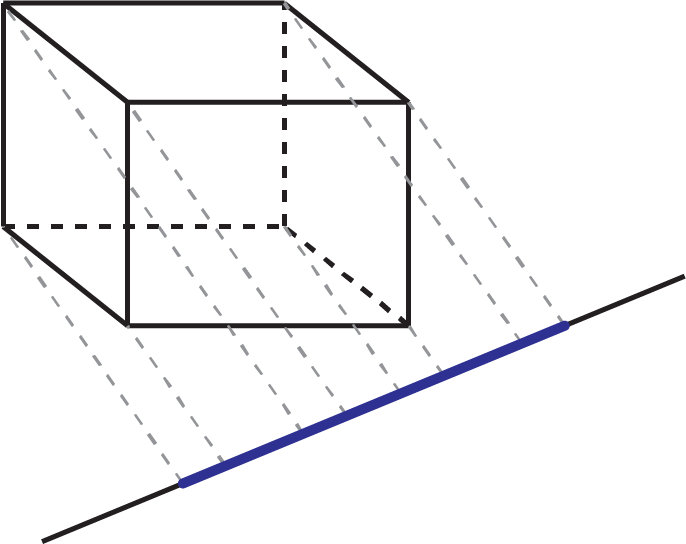
\includegraphics[scale=0.35]{Images/aabb_1d_proj.png} 
    \caption{The projection of an AABB on an axis.}
    \label{fig:aabb_1d_proj}
\end{figure}

In principle, given 2 polyhedra with 6 faces each (such as a frustum and an AABB), there should be $(6 + 6)_{normals} + (12\cdot 12)_{cross\: products} = 156$ axis to check; but, since:
\begin{itemize}
	\item The AABB has edges only in 3 different directions, and faces normals only in 3 different directions, and
	\item The frustum has edges only in 6 different directions, and faces normals only in 5 different directions
\end{itemize}
the number of checks is reduced to $(3 + 5)_{normals} + (3\cdot 6)_{cross\: products} = 26$.

\begin{figure}[H]
    \centering
    \subfloat[AABB: 3 different edges directions]{
        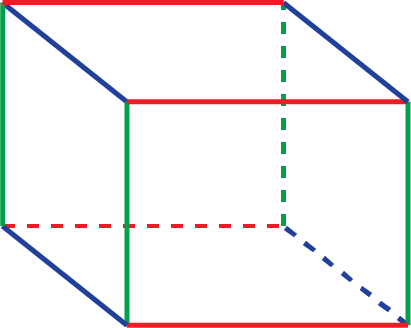
\includegraphics[scale=0.35]{Images/aabb_edges_same_dir.png}
		}
		\qquad
	\subfloat[Frustum: 6 different edges directions]{
        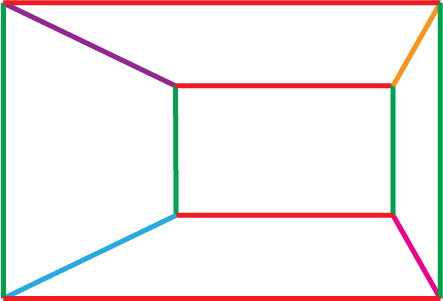
\includegraphics[scale=0.35]{Images/frustum_edges_same_dir.png}
    }
	\caption{In the figure the edges having the same direction are colored in the same color.}
    \label{fig:aabb_frustum_different_edges_directions}
\end{figure}


\subsection{1D Projections Overlapping Test}
In order to detect if the 1D projections of the 3D hulls are overlapping, we identify the outermost points of each projection (namely $A_{min}, A_{max}, B_{min}, B_{max}$) and check that $B_{min} \leq A_{max} \And B_{max} \geq A_{min}$.\\
For the AABB another optimization is possible, where we detect what points will be the outermost after the projection without actually projecting them, based on the direction of the axis:

\begin{figure}[H]
    \centering
    \subfloat[AABB vertices layout.]{
        \raisebox{-0.1\height}{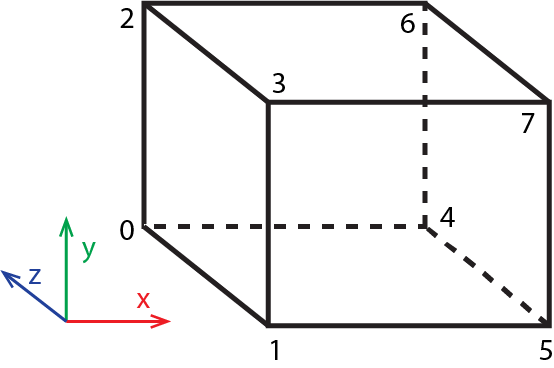
\includegraphics[scale=0.35]{Images/aabb.png}}
    }
    \quad
    \subfloat{
		\raisebox{0.5\height}{
		\begin{tabular}{| c | c |}
			\hline
			\textbf{axis direction} & \textbf{extremes} \\
			\hline \hline
			$x \geq 0 \And y \geq 0 \And z \leq 0$ & 1, 6\\
			$x \leq 0 \And y \leq 0 \And z \geq 0$ & 6, 1\\
			$x \geq 0 \And y \geq 0 \And z \geq 0$ & 0, 7\\
			$x \leq 0 \And y \leq 0 \And z \leq 0$ & 7, 0\\
			$x \geq 0 \And y \leq 0 \And z \leq 0$ & 3, 4\\
			$x \leq 0 \And y \geq 0 \And z \geq 0$ & 4, 3\\
			$x \geq 0 \And y \leq 0 \And z \geq 0$ & 2, 5\\
			$x \leq 0 \And y \geq 0 \And z \leq 0$ & 5, 2\\
			\hline
		\end{tabular}
		}
    }
    \label{fig:aabb_projected_extremes}
\end{figure}

\begin{algorithm}[H]
	\caption{Ray-AABB branchless slab intersection algorithm in 3 dimensions}
	\begin{algorithmic}[1]
		\Function{Intersect}{$frustum, aabb$}
		\If{$!intersect(frustum.aabb, aabb)$} \Comment{AABB-AABB test}
			\State \Return $false$
		\EndIf
		\Let{$axesToCheck$}{$(\perp frustum \: faces) \cup (\perp AABB \: faces) \cup (\times edges$)}
		\ForAll{$axis \in axesToCheck$}
			\Let{$frustumExtremes$}{$findFrustumExtremes(frustum, axis)$} \Comment{Returns the vertices of the frustum that, after the projection, will be the extremes}
			\Let{$aabbExtremes$}{$findAabbExtremes(aabb, axis)$} \Comment{Same as above, but uses the discussed optimization}
			\Let{$A_{min}$}{$\langle aabbExtremes.first \cdot axis \rangle$}
			\Let{$A_{max}$}{$\langle aabbExtremes.second \cdot axis \rangle$}
			\Let{$B_{min}$}{$\langle frustumExtremes.first \cdot axis \rangle$}
			\Let{$B_{max}$}{$\langle frustumExtremes.second \cdot axis \rangle$}
			\If{$!(B_{min} \leq A_{max} \And B_{max} \geq A_{min})$} 
				\State \Return $false$
			\EndIf
		\EndFor
		\State \Return $true$ \Comment{If we havent't found any axis where there is no overlap, boxes are colliding}
		\EndFunction
	\end{algorithmic}
\end{algorithm} 

\section{Point inside AABB Test} \label{sec:point_inside_aabb}
To check if a point $P$ is inside an axis-aligned bounding box in the min-max form, it is sufficient to compare its coordinates with the minimum and maximum of the AABB component-wise:
\begin{subequations}
	\begin{align*}[left=\empheqlbrace]
		min_x \leq P_x \leq max_x \\
		min_y \leq P_y \leq max_y \\
		min_z \leq P_z \leq max_z
	\end{align*}
\end{subequations}

\section{Point inside Frustum Test} \label{sec:point_inside_frustum}
It is possible to detect whether a point is inside a 3-dimensional frustum by projecting it with the perspective matrix associated with the frustum and then comparing its coordinates, as suggested by \cite{point_inside_frustum_test}.

Given the perspective matrix $\textit{M}$ associated with the frustum, we can project a point $P$ and get: $P' = \textit{M} \cdot P$; and perform the perspective division. 

$P'' = \frac{P'}{P'_w}$ $P''$ is now in normalized device coordinates (NDC) space, where the frustum is an axis-aligned bounding box that extends from $\langle -1, -1, -1 \rangle$ to $\langle 1, 1, 1 \rangle$ \footnote{Based on the convention used, it is possible that the AABB in NDC space has a different size. For example, it is common an AABB extending from $\langle -1, -1, 0 \rangle$ to $\langle 1, 1, 1 \rangle$}.

It is now immediate to see that $P$ is inside the frustum if and only if $P''$ is inside the AABB (see section \ref{sec:point_inside_aabb}).

A simple optimization allow us to avoid the perspective division. Indeed, since in homogeneous coordinates:
$$\langle x',y',z',w' \rangle = \langle \frac{x'}{w'},\frac{y'}{w'},\frac{z'}{w'},\frac{w'}{w'} \rangle = \langle x'',y'',z'',1 \rangle$$
We can change the inequalities to check whether the point is inside the frustum from:

\begin{minipage}{.4\linewidth}
	\begin{subequations}
		\begin{align*}[left=\empheqlbrace]
			-1 \leq x'' \leq 1 \\
			-1 \leq y'' \leq 1 \\
			-1 \leq z'' \leq 1
		\end{align*}
	\end{subequations}
\end{minipage}
		to:
\begin{minipage}{.4\linewidth}
	\begin{subequations}
		\begin{align*}[left=\empheqlbrace]
			-w' \leq x' \leq w' \\
			-w' \leq y' \leq w' \\
			-w' \leq z' \leq w'
		\end{align*}
	\end{subequations}
\end{minipage}

We created a 2D visual demonstration of how it is possible to detect if a point is inside a frustum at \url{https://www.geogebra.org/m/ammj5mxd}.

\section{Point inside 2D Convex Hull Test} \label{sec:point_inside_2dHull}
Given a 2D convex hull in 3-dimensional space and a 3D point laying on the same plane as the hull, it is possible to use a simple inside-outside test \cite{ray_triangle_intersection} to determine whether the point is inside the convex hull.

The main idea is that the point lays inside the convex hull if and only if it is \textit{to the right} (or \textit{to the left}, depending on the winding order) of all the edges of the hull.

In order to determine the relative position of a point and an edge $\overline{AB}$, we can look at the cross product:
$$u \times v \; where \; u = \overrightarrow{AB}, v = \overrightarrow{AP}$$

\begin{figure}[H]
    \centering
    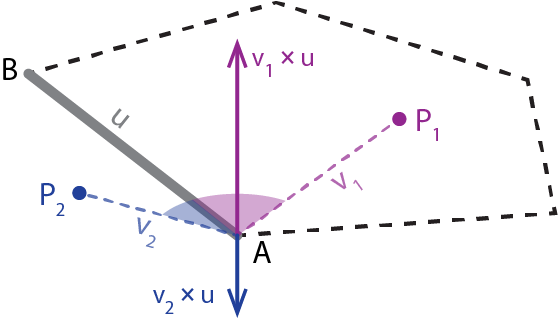
\includegraphics[scale=0.4]{Images/cross_product.png} 
    \caption{Visualization of cross product.}
    \label{fig:cross_product}
\end{figure}

Therefore the strategy to determine if a point is on the same side of all the edges of the convex hull is to compute a reference cross product, by choosing any of the edges, and then making sure that all the other cross products have the same direction. To check that 2 vectors have the same direction it is sufficient that their dot product is positive.

\begin{algorithm}[H]
	\caption{Inside-outside test between a 3D point and a 2D convex hull.} 
	\begin{algorithmic}[1]
		\Function{IsInside}{$P, hull$}
		\Let{$N$}{$number \: of \: edges \: of \: hull$}
		\Let{$u$}{$hull[0] - hull[N-1]$}
		\Let{$v$}{$P - hull[N-1]$}
		\Let{$ref$}{$u \times v$} \Comment{The reference cross product}
		\For{$0\leq i < N$}
			\Let{$u$}{$hull[i+1] - hull[i]$}
			\Let{$v$}{$P - hull[i]$}
			\Let{$cross$}{$u \times v$}
			\If{$\langle ref \cdot cross \rangle \leq 0$}
				\State \Return $false$
			\EndIf
		\EndFor
		\State \Return $true$
		\EndFunction
	\end{algorithmic}
\end{algorithm} 

\section{2D Convex Hull Culling} \label{sec:2dHull_culling}
In order to find the overlapping region between two 2D hulls in 2-dimensional space, we can proceed as illustrated in the diagram below (\cite{convex_hull_culling}):

\begin{figure}[H]
    \centering
    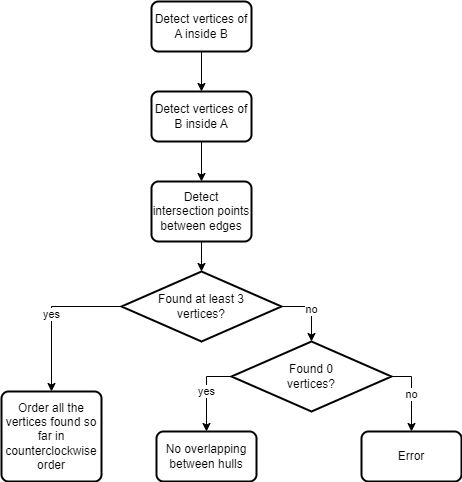
\includegraphics[scale=0.7]{Images/hull_culling.png} 
    \caption{General algorithm to find the overlapping region between two convex hulls called $A$ and $B$.}
    \label{fig:hull_culling}
\end{figure}

\begin{figure}[H]
    \centering
    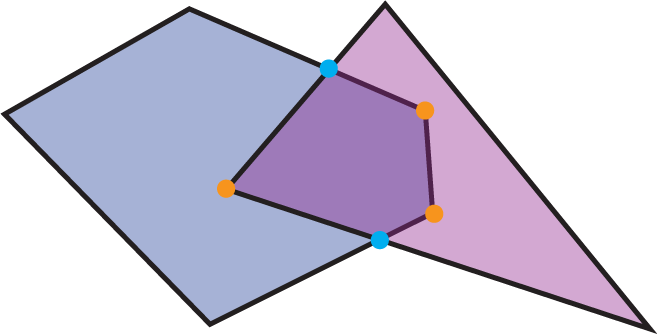
\includegraphics[scale=0.4]{Images/overlapping_hull.png} 
    \caption{Yellow vertices are found in the first 2 steps (vertices inside), whereas light blue vertices are found in the third step (edges intersections).}
    \label{fig:overlapping_hull}
\end{figure}

We'll now go through each phase and see the used algorithms.

\subsection{Vertices inside convex hull}
To find out what vertices of a hull are inside the other one we simply looped over them and used the point inside convex hull test (\ref{sec:point_inside_2dHull}).

\subsection{Edges intersections}
To detect an intersection between two segments, we first have to compute the equation of the line the segment is lying on.

Given a segment $\overline{PQ}$, the underlying line has equation:
$$A\cdot x + B\cdot y = C$$
We can then compute the parameters of the line as:
\begin{subequations}
	\begin{align*}[left=\empheqlbrace]
		A &= Q_y - P_y\\
		B &= P_x - Q_x\\
		C &= A\cdot P_x + B\cdot P_y
	\end{align*}
\end{subequations}

After we calculate the underlying line of both segments, with parameters $A_1, B_1, C_1, A_2, B_2, C_2$, we can compute the intersection point $K$ of the two lines as:
\begin{subequations}
	\begin{align*}[left=\empheqlbrace]
		\Delta &= A_1 \cdot B_2 - A_2 \cdot B_1\\
		K_x &= \frac{B_2 \cdot C_1 - B_1 \cdot C_2}{\Delta}\\
		K_y &= \frac{A_1 \cdot C_2 - A_2 \cdot C_1}{\Delta}
	\end{align*}
\end{subequations}

We are now left with the task of verifying whether the found intersection point $K$ is in between both segments' extremes. Let's call the first segment $\overline{MN}$ and the second one $\overline{PQ}$:

\begin{minipage}{.4\linewidth}
	\begin{subequations}
		\begin{align*}[left=\empheqlbrace]
			min(M_x, N_x) &\leq K_x \And\\
			max(M_x, N_x) &\geq K_x \And\\
			min(M_y, N_y) &\leq K_y \And\\
			max(M_y, N_y) &\geq K_y		
		\end{align*}
	\end{subequations}
\end{minipage}
		$And$
\begin{minipage}{.4\linewidth}
	\begin{subequations}
		\begin{align*}[left=\empheqlbrace]
			min(P_x, Q_x) &\leq K_x \And\\
			max(P_x, Q_x) &\geq K_x \And\\
			min(P_y, Q_y) &\leq K_y \And\\
			max(P_y, Q_y) &\geq K_y		
		\end{align*}
	\end{subequations}
\end{minipage}

\begin{figure}[H]
    \centering
    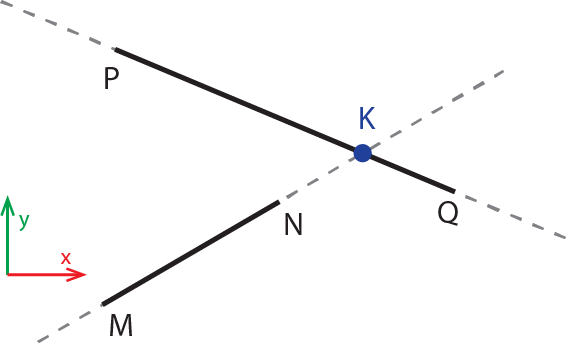
\includegraphics[scale=0.4]{Images/segments_intersection.png} 
    \caption{In this example segments do not collide because $max(M_x, N_x) = N_x \ngeq K_x$ or $max(M_y, N_y) \ngeq K_y$}
    \label{fig:cross_product}
\end{figure}

\subsection{Vertices ordering}
Given a set of unordered 2D points belonging to a convex hull, we want to sort them in a counterclockwise order, so that two consecutive vertices form an edge of the convex hull.

To do so we can compute the barycenter $O$ of the set of points that, being them part of a convex hull\footnote{We can state that the vertices we found so far make up a convex hull because the overlapping of two convex hulls is necessarily a convex hull.}, is necessarily inside the convex hull itself.

Now, for each vertex $A_k$ we can calculate the vector $\overrightarrow{OA_k}$, and sort the vertices based on $atan2(\overrightarrow{OA_k}_y, \overrightarrow{OA_K}_x)$.

The $atan2(v_y, v_x)$ function returns the angle between the positive x-axis and the vector $v=\langle v_x, v_y \rangle$. Differently from the arctangent function, the returned angle ranges in the interval $(-\pi, \pi]$, therefore is well suited for our purpose of sorting the convex hull vertices.

\begin{figure}[H]
    \centering
    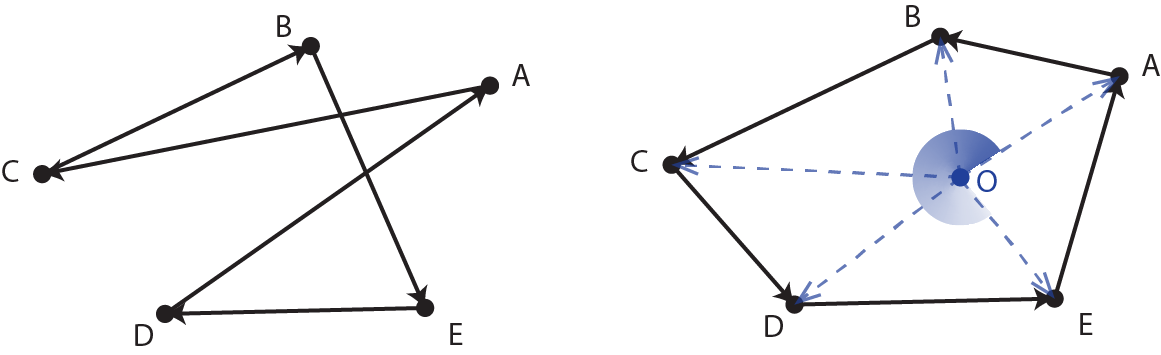
\includegraphics[scale=0.4]{Images/vertices_sorting.png} 
    \caption{Vertices of a convex hull before and after $atan2$ sorting.}
    \label{fig:vertices_sorting}
\end{figure}


% === Lists ===
\listoffigures
\listoftables

% Table of symbols
\chapter*{List of Symbols} % You have to include a chapter for your list of symbols (
\begin{table}[H]
    \centering
    \begin{tabular}{lll}
        \textbf{Symbol} & \textbf{Description} & \textbf{Unit} \\\hline\\[-9px]
        $\bm{alpha}$ & symbol 1 & km \\[2px]
    \end{tabular}
\end{table}

% === Ringraziamenti ===
\chapter*{Acknowledgements}
Ringrazio...

\cleardoublepage
\end{document}
